
\documentclass[12pt]{article}
\newcommand{\figdir}{../../Code/Rcode/Figures/AEJ_revision}
\usepackage{graphicx}
\usepackage{amsmath}

\begin{document}
\section{Comparison to BPP}
Major differences:\\
1) Data timing - the PSID measures a snapshot of consumption at the end of the year, while income is time aggregated over the year. This makes it unsuitable for measuring short-term consumption responses. To use our method, you have to make strong assumptions about how quickly consumption falls following a transitory income shock.\\
2) Actual differences in data: The PSID consumption data displays far lower sensitivity to income than Danish data, around 0.35. Another project to understand why.
3) Why was it different to previous draft? Bug in original BPP paper. Shows up for us because our data timing is very different...?
4) Why is it different to previous submission? Transitory shock vol relative to perm vol has increased as we removed less outliers. This biases the permanent MPX up as we will see shortly.
	\begin{figure} 
	\begin{centering}
		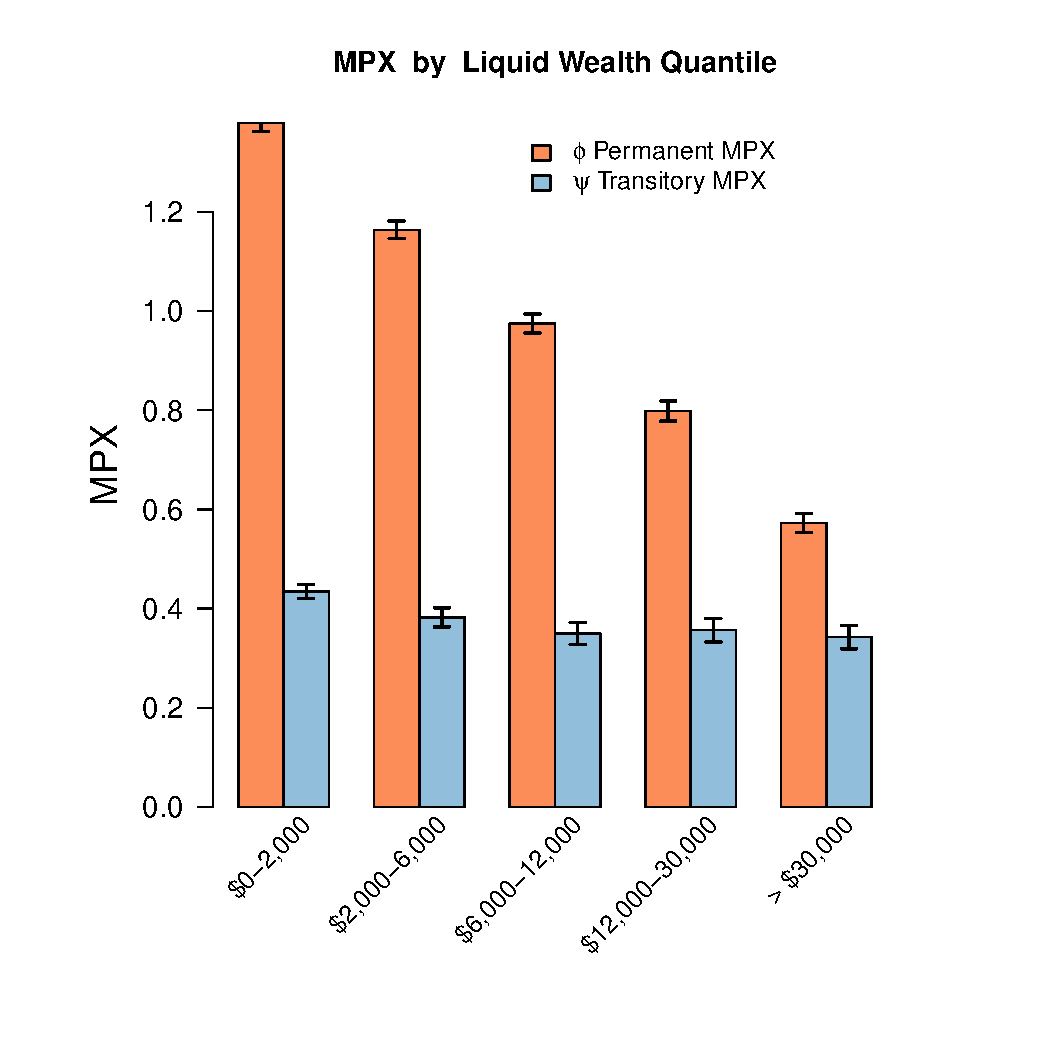
\includegraphics[scale=0.4]{\figdir/MPXByLiquidWealthBPP.pdf}
		\caption{Estimates by Liquid Wealth Quintile Obtained Using BPP's Methodology}
		\label{fig:BPP_liquid}
	\end{centering}
\end{figure}
\subsection{Random walk consumption response}
\begin{align*}
	\mathrm{Cov}(\Delta \bar{y}_T, \Delta \bar{y}_{T+1}) &= \frac{1}{6} \sigma^2_P - \sigma^2_Q &= &-\hat{\sigma}^2_{Q,BPP} \\
	\mathrm{Var}(\Delta \bar{y}_T) &= \frac{2}{3} \sigma^2_P + \sigma^2_Q &= &\hat{\sigma}^2_{P,BPP} + 2\hat{\sigma}^2_{Q,BPP} \\
	\mathrm{Cov}(\Delta \bar{c}_T, \Delta \bar{y}_{T+1}) &= \frac{1}{6} \phi \sigma^2_P  - \frac{1}{2}\psi \sigma^2_Q &= &-\hat{\psi}_{BPP} \hat{\sigma}^2_{Q,BPP} \\
	\mathrm{Cov}(\Delta \bar{c}_T, \Delta \bar{y}_T) &= \frac{2}{3} \phi \sigma^2_P  &= &\hat{\phi}_{BPP}\hat{\sigma}^2_{P,BPP} +\hat{\psi}_{BPP}\hat{\sigma}^2_{Q,BPP}
\end{align*}

\begin{align*}
	\hat{\sigma}^2_{P,BPP} &= \sigma^2_P \\
	\hat{\sigma}^2_{P,BPP} &= \sigma^2_Q - \frac{1}{6}\sigma^2_P \\
	\hat{\phi}_{BPP} &=  \frac{5}{6}\phi - \frac{1}{2}\psi\frac{\sigma^2_Q}{\sigma^2_P} \\
	\hat{\psi}_{BPP} &=  \frac{  \frac{1}{2}\psi \sigma^2_Q - \frac{1}{6}\phi \sigma^2_P}{ \sigma^2_Q - \frac{1}{6} \sigma^2_P}
\end{align*}
At $\sigma^2_P=1$, $\sigma^2_Q=1$, $\phi=0.8$, $\psi=0.8$, this recovers $\hat{\phi}_{BPP}=0.27$ and $\hat{\psi}_{BPP}=0.32$. That is, if the true model is a random walk the BPP methodology underestimates both the permanent and transitory response coefficients.
\subsection{A model with transitory consumption response}
\begin{align*}
	\mathrm{Cov}(\Delta \bar{y}_T, \Delta \bar{y}_{T+1}) &= \frac{1}{6} \sigma^2_P - \sigma^2_Q &= &-\hat{\sigma}^2_{Q,BPP} \\
	\mathrm{Var}(\Delta \bar{y}_T) &= \frac{2}{3} \sigma^2_P + 2\sigma^2_Q &= &\hat{\sigma}^2_{P,BPP} + 2\hat{\sigma}^2_{Q,BPP} \\
	\mathrm{Cov}(\Delta \bar{c}_T, \Delta \bar{y}_{T+1}) &= \frac{1}{6} \phi \sigma^2_P - \psi \sigma^2_Q &= &-\hat{\psi}_{BPP} \hat{\sigma}^2_{Q,BPP} \\
\mathrm{Cov}(\Delta \bar{c}_T, \Delta \bar{y}_T) &= \frac{2}{3} \phi \sigma^2_P + 2\psi \sigma^2_Q &= &\hat{\phi}_{BPP}\hat{\sigma}^2_{P,BPP} +\hat{\psi}_{BPP}\hat{\sigma}^2_{Q,BPP}
\end{align*}

\begin{align*}
	\hat{\sigma}^2_{P,BPP} &= \sigma^2_P \\
	\hat{\sigma}^2_{P,BPP} &= \sigma^2_Q - \frac{1}{6}\sigma^2_P \\
	\hat{\phi}_{BPP} &=  \frac{5}{6}\phi + \psi\frac{\sigma^2_Q}{\sigma^2_P}\\
	\hat{\psi}_{BPP} &=  \frac{\psi \sigma^2_Q - \frac{1}{6} \phi \sigma^2_P  }{\sigma^2_Q - \frac{1}{6} \sigma^2_P}
\end{align*}
At $\sigma^2_P=1$, $\sigma^2_Q=1$, $\phi=0.8$, $\psi=0.8$, this recovers $\hat{\phi}_{BPP}=1.47$ and $\hat{\psi}_{BPP}=0.8$. That is, under this model with parameters similar to those found for the least liquid group, the BPP method significantly overestimates the consumption response to permanent shocks, while correctly estimating the consumption response to transitory shocks.

\subsection{A model with transitory consumption response and a transitory durables response to permanent shocks}
\begin{align*}
	\mathrm{Cov}(\Delta \bar{y}_T, \Delta \bar{y}_{T+1}) &= \frac{1}{6} \sigma^2_P - \sigma^2_Q &= &-\hat{\sigma}^2_{Q,BPP} \\
	\mathrm{Var}(\Delta \bar{y}_T) &= \frac{2}{3} \sigma^2_P + 2\sigma^2_Q &= &\hat{\sigma}^2_{P,BPP} + 2\hat{\sigma}^2_{Q,BPP} \\
	\mathrm{Cov}(\Delta \bar{c}_T, \Delta \bar{y}_{T+1}) &= \frac{1}{6} \phi \sigma^2_P +\frac{1}{2}\phi_d\sigma^2_P- \psi \sigma^2_Q &= &-\hat{\psi}_{BPP} \hat{\sigma}^2_{Q,BPP} \\
	\mathrm{Cov}(\Delta \bar{c}_T, \Delta \bar{y}_T) &= \frac{2}{3} \phi \sigma^2_P + 2\psi \sigma^2_Q &= &\hat{\phi}_{BPP}\hat{\sigma}^2_{P,BPP} +\hat{\psi}_{BPP}\hat{\sigma}^2_{Q,BPP}
\end{align*}

\begin{align*}
	\hat{\sigma}^2_{P,BPP} &= \sigma^2_P \\
	\hat{\sigma}^2_{P,BPP} &= \sigma^2_Q - \frac{1}{6}\sigma^2_P \\
	\hat{\phi}_{BPP} &=  \frac{5}{6}\phi + \frac{1}{2}\phi_d + \psi\frac{\sigma^2_Q}{\sigma^2_P}\\
	\hat{\psi}_{BPP} &=  \frac{\psi \sigma^2_Q - \frac{1}{6} \phi \sigma^2_P - \frac{1}{2}\phi_d\sigma^2_P }{\sigma^2_Q - \frac{1}{6} \sigma^2_P}
\end{align*}
At $\sigma^2_P=1$, $\sigma^2_Q=1$, $\phi=0.8$, $\psi=0.8$, and  $\phi_d=0.5$, this recovers $\hat{\phi}_{BPP}=1.72$ and $\hat{\psi}_{BPP}=0.5$, close to that obtained empirically for the households in the lowest quintile of liquid wealth.

\subsection{Conclusion}
The BPP method is incredibly sensitive to timing and short term dynamics.\\
The empirical evidence is consistent with a model in which permanent shocks are associated with initial durable expenditure. \\
Much more work can be done in this direction. Indeed I am working on this.
	
\end{document}